\documentclass[12pt,a4paper]{book}
\usepackage[left=2cm, right=2cm, top=2cm, bottom=2cm]{geometry}  
\usepackage[UTF8]{ctex}                                                      
%%
\usepackage{indentfirst,setspace,microtype}  
\linespread{1.5}          
%%  
\usepackage{amssymb,amsfonts,amsmath,bm,showlabels}                          
\allowdisplaybreaks                                  
%%
\usepackage{graphicx,subfigure,caption,enumitem,epstopdf,epsfig,wrapfig,tikz}   
\graphicspath{{figure/}}
%%
\usepackage{hyperref,cite,color,xcolor,framed}  
\hypersetup{colorlinks=true,citecolor={red},linkcolor={blue}} 
%%
\usepackage{changes}
\definechangesauthor{red}
\colorlet{Changes@Color}{red}
%% 
\usepackage{titlesec}
\titleformat{\paragraph}[hang]{}{\theparagraph \quad}{0pt}{}  
\titleformat{\subparagraph}[hang]{}{\thesubparagraph \quad}{0pt}{}         
\setcounter{tocdepth}{5}  
\setcounter{secnumdepth}{5} 
%%
%\usepackage{draftwatermark}
%\SetWatermarkText{内部使用} % the Text
%\SetWatermarkLightness{0.9} % the lightness from 0 to 1, default 0.8
%\SetWatermarkScale{0.5} % the scale, default 1.2
%% others
\usepackage{pifont,listings,framed}    
%% newcommand
% \newcommand{\mathcolorbox}[2]{\colorbox{#1}{$ #2$}}
\newcommand{\mathcolorbox}[2]{\colorbox{#1}{$\displaystyle #2$}}
\newcommand\hl[1]{\bgroup\markoverwith{\textcolor{#1}{\rule[-.5ex]{2pt}{2.5ex}}}\ULon}

\usepackage{tikz}
\usetikzlibrary{tikzmark}

% title, author, date
\title{\LARGE\bfseries\songti 学习笔记}

\author{ \kaishu 平安喜乐
		\thanks{常怀感恩之心!} \\[0.5ex] % 在第一页左下角加感谢
		}

\date{\small\itshape Last update: \today}


\begin{document}
\songti
% \youyuan 
% \kaishus
% \fangsong

\maketitle 
\clearpage

\tableofcontents  
\clearpage




\clearpage
\chapter*{8 有限元分析:理论和实现}

\section*{8.1 静力线弹性有限元}


\subsection*{8.1.5 有限元的简单一维实现}


在描述一个完全通用的三维有限元实现之前,我们将用一个简单的一维例子来说明所有的关键思想。考虑一根长的线弹性杆,如图8.3所示。假设:

\begin{enumerate}
    \item 杆的剪切模量为 $\mu$,泊松比为 $\nu$
    \item 杆的横截面积为 $h\times h$,长度为 $L$
    \item 杆的所有侧边都受到约束,所以 $u_2=u_3=0$
    \item 杆受到体力 $\bm{b} = b(x_1) \bm{e}_1$
    \item 杆的两端或者有载荷或者被约束,因此,边界条件或者是 $t_1(0) = t^*(0), t_1(L) = t^*(L)$, 或者是 $u_1(0) = u^*(0), u_1(L) = u^*(L)$,当 $x=0$ 和 $x=L$ 时。
\end{enumerate}

那么,对于这个一维例子,有限元方程退化为
\begin{equation*}
    \begin{aligned}
        K_{ab} u_1^b = F^a,
    \end{aligned}
\end{equation*}
其中
\begin{equation*}
    \begin{aligned}
        K_{a b} & = h^{2} \int_{0}^{L} \frac{2 \mu(1-v)}{1-2 v} \frac{\partial N^{a}\left(x_{1}\right)}{\partial x_{1}} \frac{\partial N^{b}\left(x_{1}\right)}{\partial x_{1}} d x_{1}
    \end{aligned}
\end{equation*}
%
\begin{equation*}
    \begin{aligned}
        F^{a}=h^{2} \int_{0}^{L} b N^{a}\left(x_{1}\right) d x_{1}+h^{2} t_{1}^{*}(0) N^{a}(0)+h^{2} t^{*}(L) N^{a}(L) .
    \end{aligned}
\end{equation*}

显然,我们可以选择任何插值方案,计算必要的积分,并求解得到的方程组来计算解。然而,使用分段拉格朗日插值格式和高斯数值积分格式,已被证明是极为方便的。





% ---


为了实现拉格朗日插值方案,我们将区域 $ 0 \leq  x_1 \leq L $ 细分为一系列单元,如图8.4所示。每个单元以两个节点为界,也可以包含一个或多个内部节点。根据单元节点位移,插值得到单元内部位移场。因此,我们将在两节点单元上使用线性插值,在三节点单元上使用二次插值,等等。

\begin{equation*}
    \begin{aligned}
        u_{1}\left(\xi_{1}\right)=\sum_{a=1}^{N_{e}} N^{a}\left(\xi_{1}\right) u_{1}^{a}
    \end{aligned}
\end{equation*}


一般的线性和二次一维单元如表8.1所示。对于线性单元,单元上的节点被编号为1和2。对于二次单元,单元上的节点被编号为1,2,3。假设该单元位于 $-1 \leq \xi_1 \leq 1$ 的区域内。那么,单元内的位移被插值为
\begin{equation*}
    \begin{aligned}
        u_{1}\left(\xi_{1}\right)=\sum_{a=1}^{N_{e}} N^{a}\left(\xi_{1}\right) u_{1}^{a}u_{1}\left(\xi_{1}\right)=\sum_{a=1}^{N_{e}} N^{a}\left(\xi_{1}\right) u_{1}^{a},
    \end{aligned}
\end{equation*}
其中,$N_e$ 表示单元上的节点数,$u_1^a$ 表示每个节点上的位移值,形状函数在表中给出。


当然,对于所有单元,实际节点坐标并不位于 $-1, +1, 0$。对于一个一般的单元,我们将这个特殊的单元映射到感兴趣的区域。一个特别方便的方法是设置
\begin{equation*}
    \begin{aligned}
        x_{1}\left(\xi_{1}\right)=\sum_{a=1}^{N_{e}} N^{a}\left(\xi_{1}\right) x_{1}^{a}
    \end{aligned}
\end{equation*}
其中 $x_1^a$ 表示单元上每个节点的坐标,$N_e$ 是单元节点数(2或3)。使用相同形函数插值位移和位置的单元称为等参单元。

接下来,我们需要设计一种方法来对刚度矩阵和力矢量的表达式进行积分。显然,我们可以将积分进行分割,依次对每个元素积分:

\begin{equation*}
    \begin{aligned}
        K_{a b}=\sum_{l=1}^{N_{\text {lmn }}} h^{2} \int_{x 0}^{x 1} \frac{2 \mu(1-v)}{1-2 v} \frac{\partial N^{a}\left(x_{1}\right)}{\partial x_{1}} \frac{\partial N^{b}\left(x_{1}\right)}{\partial x_{1}} d x_{1}
    \end{aligned}
\end{equation*}


\begin{equation*}
    \begin{aligned}
        F^{a}=\sum_{l=1}^{N_{l m n}} h^{2} \int_{x 0}^{x 1} b N^{a}\left(x_{1}\right) d x_{1}+h^{2} t_{i}^{*} N^{a}(0)+h^{2} t_{i}^{*} N^{a}(L)
    \end{aligned}
\end{equation*}

\begin{figure}[!ht]
	\centering
	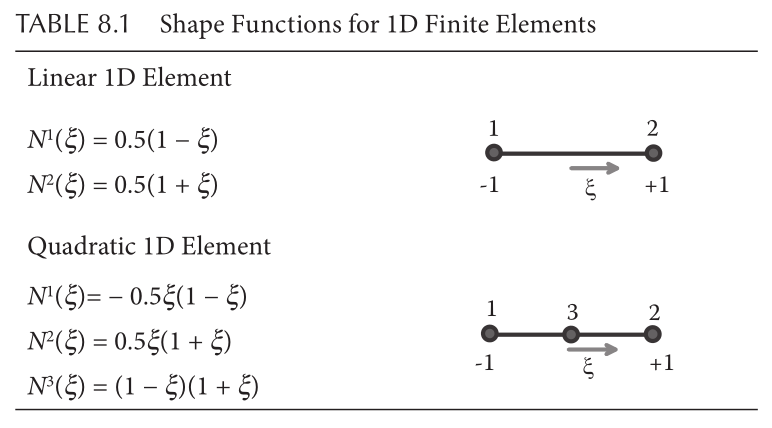
\includegraphics[width=0.45\textwidth]{Table_8_1.png}
	%%\caption{}
\end{figure}
其中 $N_{lmn}$ 是单元的总数,$x_0$ 和 $x_1$ 表示第 $l$ 个单元端点的坐标。我们现在注意到我们的插值方案的一个吸引人的特点。因为第 $l$ 个单元所在区域的位移完全由该单元上的节点值决定,所以第 $l$ 个单元上的积分只取决于与该单元的节点相关的形函数。因此,对于每个单元,我们可以定义单元刚度矩阵和单元力矩阵,
\begin{equation*}
    \begin{aligned}
        k_{a b}=h^{2} \int_{x 0}^{x 1} \frac{2 \mu(1-v)}{1-2 v} \frac{\partial N^{a}\left(x_{1}\right)}{\partial x_{1}} \frac{\partial N^{b}\left(x_{1}\right)}{\partial x_{1}} d x_{1}
        \qquad
        f^{a}=h^{2} \int_{x 0}^{x 1} b N^{a}\left(x_{1}\right) d x_{1},
    \end{aligned}
\end{equation*}
其取决于几何,插值函数和单元的材料属性。第一个和最后一个单元对单元力向量有来自边界项 $h^2 t^* N^a(0), h^2 t^* N^a(L)$ 额外的贡献。全局刚度矩阵由所有单元刚度矩阵之和计算:
\begin{equation*}
    \begin{aligned}
        K_{a b}=\sum_{l=1}^{N_{l m n}} k_{a b} 
        \qquad
        F^{a}=\sum_{l=1}^{N_{\operatorname{lmn}}} f^{a}+h^{2} t^{*} N^{a}(0)+h^{2} t^{*} N^{a}(L)
    \end{aligned}
\end{equation*}


最后,我们需要设计一种计算每个单元刚度矩阵积分的方法。将积分域映射到 $[-1,+1]$ 并根据无量纲化坐标 $\xi$ 积分是很方便的。因此,
\begin{equation*}
    \begin{aligned}
        k_{a b}=h^{2} \int_{-1}^{+1} \frac{2 \mu(1-v)}{1-2 v} \frac{\partial N^{a}(x)}{\partial x} \frac{\partial N^{b}(x)}{\partial x} J d \xi \quad f^{a}=h^{2} \int_{-1}^{+1} b N^{a}\left(x_{1}\right) J d \xi,
    \end{aligned}
\end{equation*}
其中 $J=|\partial x/d \xi|$ 是与映射相关的雅克比矩阵,可被计算为
\begin{equation*}
    \begin{aligned}
        \frac{\partial x}{\partial \xi}=\frac{\partial}{\partial \xi} \sum_{a=1}^{N_{e}} N^{a}(\xi) x^{a}=\sum_{a=1}^{N_{e}} \frac{\partial N^{a}}{\partial \xi} x^{a}
    \end{aligned}
\end{equation*}
请注意,映射也使我们能够计算单元刚度矩阵中形函数的导数
\begin{equation*}
    \begin{aligned}
        \frac{\partial N^{a}}{\partial x}=\frac{\partial N^{a}}{\partial \xi} \frac{\partial \xi}{\partial x}=\frac{\partial N^{a}}{\partial \xi}\left[\frac{\partial x}{\partial \xi}\right]^{-1}
    \end{aligned}
\end{equation*}

最后,请注意,可以使用数值求积公式计算积分,如下所示
\begin{equation*}
    \begin{aligned}
        \int_{-1}^{+1} g(\xi) d \xi \approx \sum_{I=1}^{M} w_{I} g\left(\xi^{(I)}\right)
    \end{aligned}
\end{equation*}
其中 $\xi^{(I)} = 1...M$ 表示区域 $[-1,+1]$ 中的积分点集合,$w_I$ 是积分权重的集合,选择积分权重是为了使近似尽可能准确。表8.2给出了 $M = 1,2,3$ 的值。存在高阶积分方案,但只对高阶单元有要求。对于上述线性一维单元,单个积分点足以准确地计算其刚度。类似地,对于二次单元,两个积分点就足够了。

% 

% \begin{equation*}
%     \begin{aligned}


%     \end{aligned}
% \end{equation*}


\bibliographystyle{ieeetr}
\bibliography{reference}




\end{document}





